\chapter{(S) SOR\label{chapter:sor}}
\rhead{(S) SOR}
\begin{refsection}
\chapterauthor{Felix Hofer}

\section{Einf"uhrung}
``Successive Overrelaxation'' -- kurz SOR -- bezeichnet eine
\index{SOR}
\index{Overrelaxation}
\index{Overrelaxation!Successive}
Modifikation bestehender iterativer Approximationsverfahren, welche
die Konvergenzgeschwindigkeit gegen"uber den unmodifizierten Verfahren
erh"ohen soll. Das Prinzip wird oft anhand des Gauss-Seidel-Algorithmus
illustriert, kann aber genauso gut auch auf andere iterative
Approximationsverfahren zur L"osung linearer Gleichungssystemen angewendet
werden.
\index{Relaxationsparameter}

Die grundlegende Idee hinter dem SOR-Prinzip ist, dass eine einmal
eingeschlagene Richtung hin zur schlussendlichen L"osung so falsch
nicht sein kann, weshalb man gleich einen etwas gr"osseren Schritt
in die entsprechende Richtung wagt (daher auch die Bezeichnung
\textbf{over}relaxation). Zus"atzlich l"asst man den vorhergehenden
Iterationsschritt in die Berechnung der neuen Approximation der echten
L"osung mit einfliessen.

Wie stark man den neuen Schritt ``"uberrelaxiert'' bzw. wie stark der
vorhergehende Iterationsschritt noch in die Berechnung mit einfliesst
steuert man mittels des sogenannten ("Uber-) Relaxationsparameters
$\omega$.
	
\section{SOR-Algorithmus\label{sec: SOR-Alg.}}
Zur Illustration des SOR-Algorithmus und zur Herleitung einer
Iterationsformel nehmen wir die unmodifizierte Variante von
Gauss-Seidel (siehe Kapitel \ref{section-gauss-seidel}, Gleichung
\ref{gauss-seidel-iteration}) als Vorlage, die den unrelaxierten
Iterationsschritt eines einzelnen $x_i$ repr"asentiert:
\begin{equation} \label{eq: G.-S.-It.formel}
	x_i^{(k+1)} = \frac{1}{a_{ii}}\left(b_i-\sum\limits_{j=1}^{i-1} a_{ij}x_j^{(k+1)}-\sum\limits_{j=i+1}^na_{ij}x_j^{(k)}\right)
\end{equation}
Dieser Iterationsschritt wird nun mit $\omega$ relaxiert -- das heisst
gestreckt. Zus"atzlich l"asst man, abh"angig von $\omega$, das $x_i$
des letzten Iterationsschrittes in die Berechnung des neuen $x_i$ mit
einfliessen, was zur folgenden, f"ur SOR modifizierten Iterationsformel
von Gauss-Seidel f"uhrt:
\begin{equation} \label{eq: SOR-It.formel1}
	x_i^{(k+1)} = \frac{\boldsymbol{\textcolor{red}{\omega}}}{a_{ii}}\left(b_i-\sum\limits_{j=1}^{i-1}a_{ij}x_j^{(k+1)}-\sum\limits_{j=i+1}^n a_{ij}x_j^{(k)}\right)\boldsymbol{\textcolor{red}{+(1-\omega)x_i^{(k)}}}
\end{equation}
Auf die Wahl des Wertes f"ur $\omega$ wird sp"ater eingegangen.
		
\subsection{Herleitung von Matrix-Zerlegung und Iterationsformel \label{subsec: SOR-Herleitung}}
Wie Jacobi und Gauss-Seidel basiert auch der SOR-Algorithmus auf einer
Matrix-Aufteilung in ``einfach'' invertierbare Matrizen wie zum Beispiel
Dreiecks- oder Diagonalmatrizen.

Um auf die schlussendliche Matrix-Formel zu kommen, wird obige
Summenformel (\ref{eq: SOR-It.formel1}) nach $x_i^{(k)}$ und $x_i^{(k+1)}$
getrennt und anschliessend mit $a_{ii}$ multipliziert, damit in der
endg"ultigen Iterationsformel dann nicht $D^{-1}$ vorkommt:
\begin{equation} \label{eq: SOR-It.formel2}
	%for\ i=1, ..., n\\
	%\left[
	%\underbrace{
	a_{ii}x_i^{(k+1)} %}_{\substack{Dx^{(k+1)}}}
	+\omega %\underbrace{
	\sum\limits_{j=1}^{i-1} a_{ij}x_j^{(k+1)} %}_{\substack{Lx^{(k+1)}}}
 = \omega b_i- \omega %\underbrace{
 \sum\limits_{j=i+1}^n a_{ij}x_j^{(k)} %}_{\substack{Ux^{(k)}}}
 +(1-\omega)	%\underbrace{
	a_{ii}x_i^{(k)} %}_{\substack{Dx^{(k)}}}
	%\right.
\end{equation}
Wenn man nun mit Gleichung (\ref{eq: SOR-It.formel2}) einen kompletten
Iterationsschritt f"ur s"amtliche Vektor-Komponenten $x_i$ mit $i=1,\
...,\ n$ ausf"uhrt, so kann man einzelne Teile der Summenformel
durch Teilmengen der Ausgangsmatrix A audr"ucken und diese so als
vereinfachte Matrix-Gleichung umschreiben (vergleiche dazu auch Kapitel
\ref{section-matrix-aufteilung}, Gleichung \ref{gauss-seidel:herleitung}):
\begin{equation} \label{eq: SOR-It.formel3}
Dx^{(k+1)}+\omega Lx^{(k+1)}=\omega b-\omega Ux^{(k)}+(1-\omega)\cdot Dx^{(k)}
\end{equation}
Wobei $D$ der Diagonale von $A$ entspricht, $L$ dem Teil unterhalb
der Diagonale und $U$ dem Teil oberhalb. Somit ergibt sich f"ur die
Ausgangsmatrix A mit SOR folgende Zerlegung, in der zum Beispiel auch
das Jacobi- oder das Gauss-Seidel-Verfahren dargestellt werden k"onnen:
\begin{equation} \label{eq: SOR Matrix-Splitting}
A=D+L+U
\end{equation}
Klammert man in Gleichung (\ref{eq: SOR-It.formel3}) nun noch $x^{(k)}$
und $x^{(k+1)}$ aus und multipliziert diese dann mit $(D+\omega
L)^{-1}$, so erh"alt man die endg"ultige SOR-Iterationsformel f"ur den
Gauss-Seidel-Algorithmus als Matrix-Gleichung:
\begin{equation} \label{eq: SOR-It.formel}
x^{(k+1)}=\underbrace{(D+\omega L)^{-1}}_{\substack{M^{-1}}}\cdot(\omega b-\underbrace{[\omega U+(\omega-1)\cdot D]}_{\substack{N}}\cdot x^{(k)})
\end{equation}
		
\section{Wahl des optimalen Relaxationsparameters}
Die Wahl des ("Uber-) Relaxationsparameters $\omega$ hat einen
entscheidenden Einfluss auf die Konvergenzgeschwindigkeit des
SOR-Verfahrens. Mit ihm kann sie gegen"uber dem unrelaxierten Algorithmus
enorm gesteigert, bei Wahl eines suboptimalen $\omega$ aber auch
verringert werden (siehe Kapitel \ref{subsec: Konv.geschw.analyse}). Bei
Wahl eines falschen $\omega$ divergiert das SOR-Verfahren.

Da $\omega$ jedoch von der jeweiligen Ausgangsmatrix $A$ abh"angig ist,
lassen sich leider keine allgemein g"ultigen Aussagen "uber die Wahl
des optimalen $\omega$ machen.

Setzt man in der SOR-Iterationsformel (Gleichung \ref{eq: SOR-It.formel})
f"ur $\omega$ genau 1 ein, so ergibt sich die urspr"ungliche Variante
des unmodifizierten Algorithmus (vergleiche dazu auch die Gleichungen
\ref{eq: G.-S.-It.formel} und \ref{eq: SOR-It.formel1}).

Im Normalfall wird man einen "Uberrelaxationsparameter $(\omega > 1$)
w"ahlen, um die Schrittweite gegen"uber dem unrelaxierten Algorithmus
zu vergr"ossern und so die Konvergenz zu beschleunigen.

Es ist aber auch denkbar, den Relaxationsparameter $\omega$ kleiner
als 1 zu w"ahlen, um so die Berechnung eines ansonsten leicht
divergierenden Problems zu stabilisieren. Allerdings wird dadurch die
Konvergenzgeschwindigkeit verringert, da man auf diese Weise einen
kleineren Schritt in Richtung der echten L"osung macht als mit dem
unmodifizierten Algorithmus. Daf"ur fliesst der letzte Iterationsschritt
noch mehr in die Berechnung mit ein.

In der Praxis werden zur Absch"atzung des optimalen Wertes f"ur $\omega$
meist heuristische Verfahren angewendet. F"ur verschiedene bekannte
Probleme gibt es aber mittlerweile auch Formeln, mit denen sich das
optimale $\omega$ ann"ahernd oder auch exakt berechnen l"asst.

F"ur einige bestimmte Matrix-Arten, wie zum Beispiel tridiagonale
Blockmatrizen, l"asst sich es sich n"amlich direkt berechnen. Oft ist die
Berechnung entsprechender Formeln oder aber auch nur schon Teilen daraus
jedoch so aufw"andig, dass auch hier anfangs wieder auf heuristische
Verfahren zur"uckgegriffen werden muss.

Im Jahre 1947 hat der russisch-deutsch-schweizerische Mathematiker
Alexander Markowitsch Ostrowski \cite{AlexanderMarkowitschOstrowski}
\index{Ostrovski, Alexander Markowitsch}
bewiesen, dass der SOR-Algorithmus f"ur positiv definitive
Ausgangsmatrizen A konvergiert, wenn $\omega \in (0,2)$. In diesem Falle
ist also der Spektralradius $\rho(G) < 1$ mit
\begin{equation} \label{Spektralradius}
G=M^{-1}N,\hspace{.1\textwidth}
M=D+\omega L,\hspace{.1\textwidth}
N=\omega U+(\omega-1)\cdot D.
\end{equation}
Im Jahre 1958 hat ausserdem der kanadische Mathematiker und Informatiker
William Kahan \cite{WilliamKahan} bewiesen, dass f"ur den SOR-Algorithmus
\index{Kahan, William}
mit $\omega < 0$ oder $\omega > 2$ keine Konvergenz mehr vorliegt.
			
\subsection{Analyse der Konvergenzgeschwindigkeit \label{subsec:
Konv.geschw.analyse}}
Zur Analyse der Konvergenzgeschwindigkeit der verschiedenen
Verfahren und $\omega$ wurde folgendes Zahlenbeispiel aus Kapitel
\ref{section-matrix-aufteilung} verwendet:
\begin{equation} \label{G.-S.-Ex.}
A=
\begin{pmatrix}
	2 & 1 & 0 \\
	2 & 3 & 2 \\
	0 & 1 & 2
\end{pmatrix},
			\qquad
b=
\begin{pmatrix}
	1 \\
	2 \\
	3
\end{pmatrix},
\qquad
x_0=
\begin{pmatrix}
	0 \\
	0 \\
	0
\end{pmatrix}
\end{equation}
Der Spektralradius $\rho(G)$ wurde mit Matlab als
\texttt{max(abs(eig(G)))} berechnet. Das optimale $\omega$ wurde
ebenfalls in Matlab mit einer for-Schleife in Hundertstel-Schritten
zwischen $\omega=1, ..., 2$ gesucht:
\begin{figure}[!ht]\centering
%	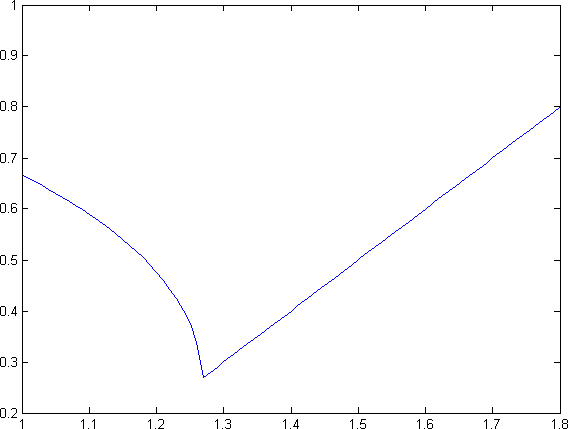
\includegraphics[width=0.66\textwidth]{img/Spektralradius.png}
\caption{Spektralradius des Problems in Abh"angigkeit von $\omega$.}
\label{fig:Spekt.rad.vs.omega}
\end{figure}

Vergleicht man nun den Spektralradius der verschiedenen Verfahren und $\omega$, kann man deutliche Unterschiede erkennen:
\begin{figure}[!ht]\centering
%	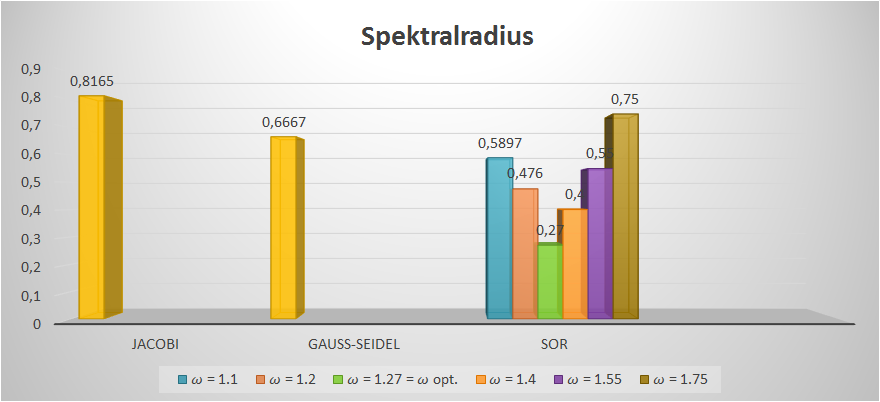
\includegraphics[width=0.75\textwidth]{img/Spektralradius_Diagramm.png}
\caption{Spektralradien verschiedener Verfahren und $\omega$.}
\label{fig:Spekt.rad. Diagr.}
\end{figure}\\

Mit der Formel 
\begin{equation} \label{eq: Accuracy}
n=\frac{-k \log{(10)}}{\log{(\rho(G))}}
\end{equation}
wurde die notwendige Anzahl Iterationsschritte f"ur eine Genauigkeit von
$k=4$ Nachkommastellen berechnet und ebenfalls f"ur die verschiedenen
Verfahren und $\omega$ visualisiert:
\begin{figure}[!ht]\centering
%	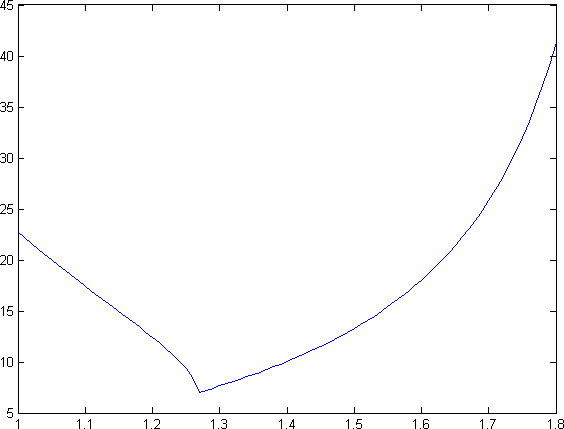
\includegraphics[width=0.66\textwidth]{img/NumIt.png}
\caption{Notwendige Anzahl Iterationen f"ur  eine Genauigkeit von 4 Nachkommastellen in Abh"angigkeit von $\omega$.}
\label{fig:Spekt.rad.vs.Anz.It.}
\end{figure}
\begin{figure}[!ht]\centering
%	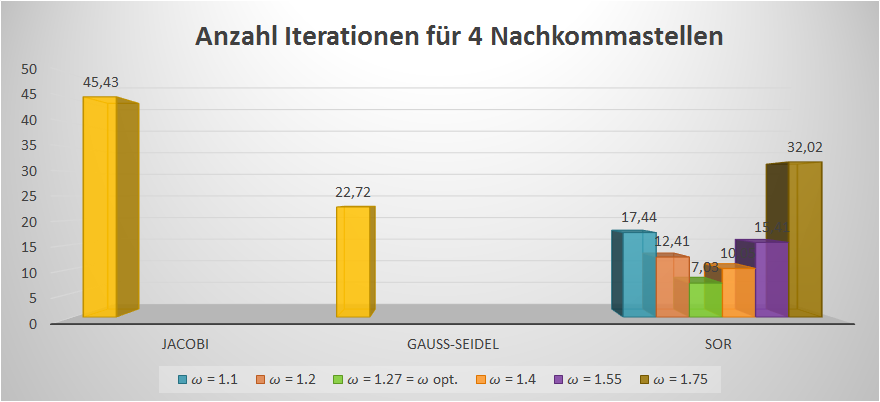
\includegraphics[width=0.75\textwidth]{img/NumIt_Diagramm.png}
\caption{Notwendige Anzahl Iterationen f"ur  eine Genauigkeit von 4 Nachkommastellen verschiedener Verfahren und $\omega$.}
\label{fig:It.vs.omega}
\end{figure}

Wie nicht anders zu erwarten sind auch hier deutliche Unterschiede zu erkennen.
		
\subsection{Visualisierung der Iterationsschritte}
Die folgenden Visualisierungen zeigen die effektiv errechneten
Iterationsschritte mit dem Jacobi-, dem Gauss-Seidel- und dem in
Kapitel \ref{sec: SOR-Alg.} beschriebenen SOR-Verfahren in einem 2D-
bzw. 3D-Koordinatensystsem.

Anhand diesen kann man gut erkennen, wie man beim SOR-Verfahren mit
einem zu grossen $\omega$ "uber das eigentliche Ziel hinausschiesst,
bei Wahl eines guten $\omega$ mit gr"osseren Schritten gegenüber Jacobi
und Gauss-Seidel aber auch schneller dort angelangt.

Wie bei den vorhergehenden zeigen auch die folgenden Visualisierungen
die Schritte f"ur eine Genauigkeit von 4 Nachkommastellen.
			
\subsubsection{2D-Beispiel}
Die folgenden Visualisierungen wurden anhand dem Zahlenbeispiel zum
Jacobi-Algorithmus aus Kapitel \ref{Algorithmus!Jacobi} erstellt.
\begin{figure}[!ht]\centering
%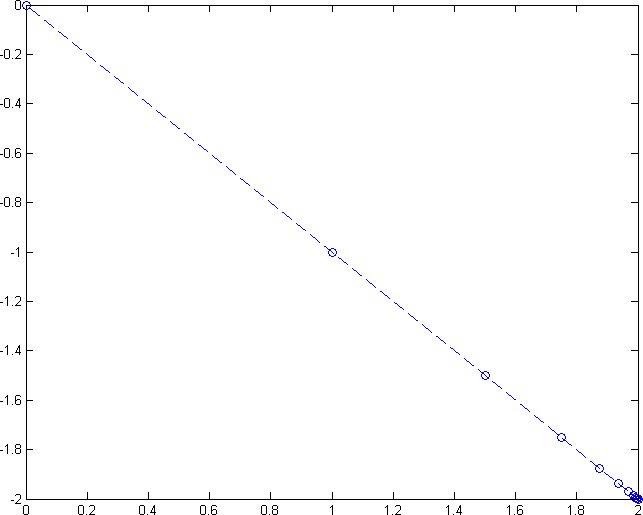
\includegraphics[width=0.5\textwidth]{img/Jac_2D_14It.png}
\caption{Jacobi, 14 Iterationen.}
\label{fig:Jac. 2D Bsp}
\end{figure}
\begin{figure}[!ht]\centering
%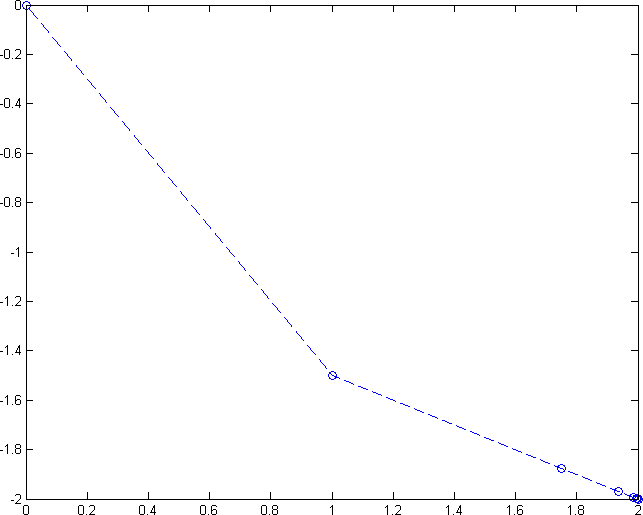
\includegraphics[width=0.5\textwidth]{img/G_S_2D_7It.png}
\caption{Gauss-Seidel, 7 Iterationen.}
\label{fig:G.-S. 2D Bsp}
\end{figure}
\begin{figure}[!ht]\centering
%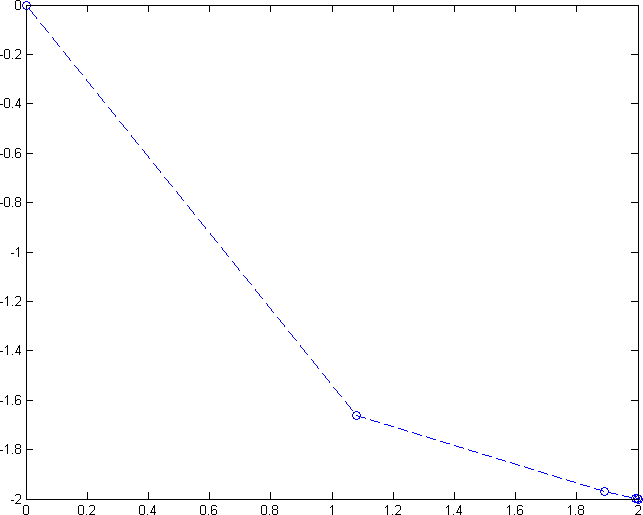
\includegraphics[width=0.5\textwidth]{img/SOR_2D_4_It_w_1_08.png}
\caption{SOR, 4 Iterationen, $\omega=1.08=\omega_{\text{opt}}$}
\label{fig:SOR w=1.08= 2D Bsp}
\end{figure}

\begin{figure}[!ht]\centering
%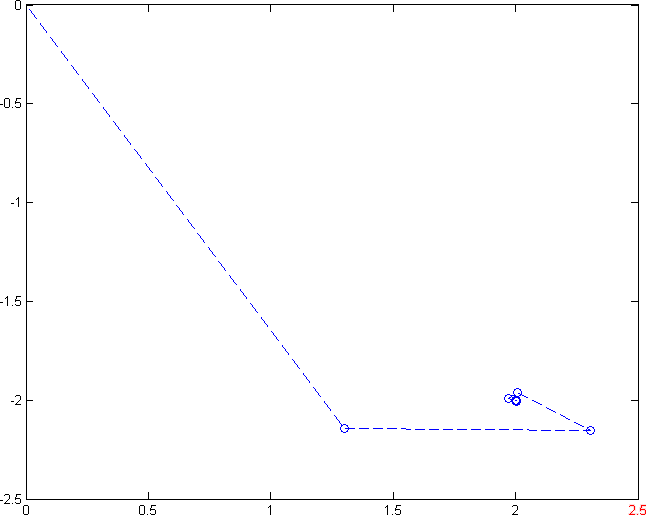
\includegraphics[width=0.5\textwidth]{img/SOR_2D_8_It_w_1_3.png}
\caption{SOR, 8 Iterationen, $\omega=1.3$}
\label{fig:SOR w=1.3 2D Bsp}
\end{figure}
\begin{figure}[!ht]\centering
%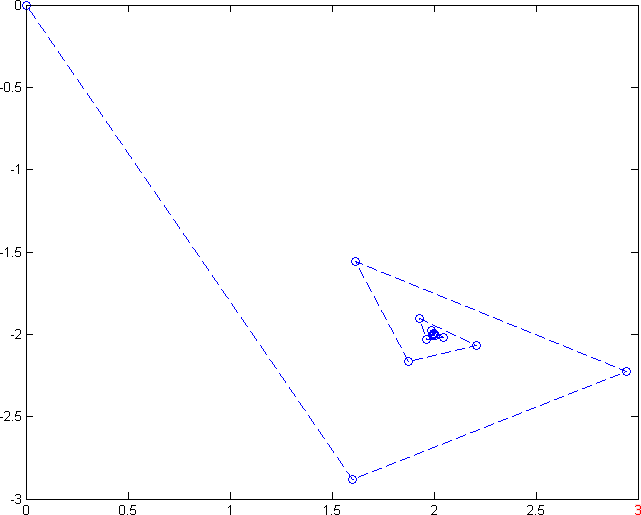
\includegraphics[width=0.5\textwidth]{img/SOR_2D_19_It_w_1_6.png}
\caption{SOR, 19 Iterationen, $\omega=1.6$}
\label{fig:SOR w=1.6 2D Bsp}
\end{figure}
	
\subsubsection{3D-Beispiel}
Die folgenden Visualisierungen wurden anhand dem Zahlenbeispiel zum
Gauss-Seidel-Algorithmus aus Kapitel \ref{section-matrix-aufteilung}
(bzw. Kapitel \ref{subsec: Konv.geschw.analyse}) erstellt.
\begin{figure}[!ht]\centering
%	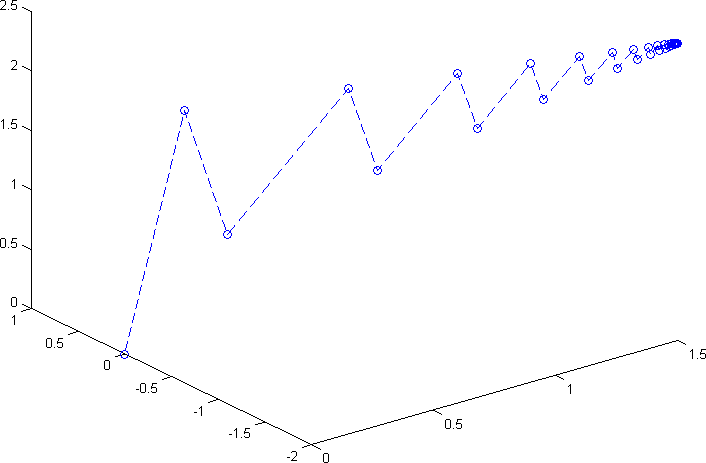
\includegraphics[width=0.5\textwidth]{img/Jacobi_3D_46_It.png}
	\caption{Jacobi, 46 Iterationen.}
	\label{fig:Jac. 3D Bsp}
\end{figure}
\begin{figure}[!ht]\centering
%	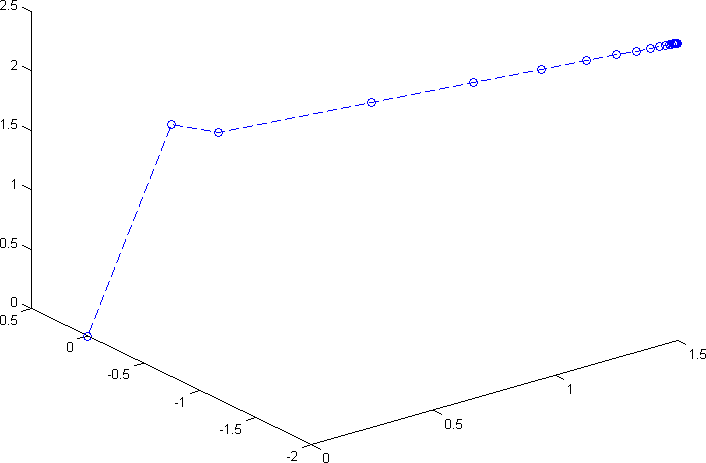
\includegraphics[width=0.5\textwidth]{img/G_S_3D_23_It.png}
	\caption{Gauss-Seidel, 23 Iterationen.}
	\label{fig:G.-S. 3D Bsp}
\end{figure}
\begin{figure}[!ht]\centering
%	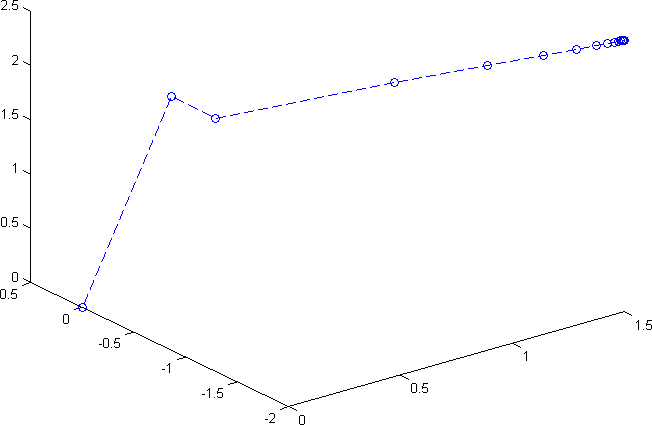
\includegraphics[width=0.5\textwidth]{img/SOR_3D_18_It_w_1_1.png}
	\caption{SOR, 18 Iterationen, $\omega=1.1$}
	\label{fig:SOR w=1.1 3D Bsp}
\end{figure}
\begin{figure}[!ht]\centering
%	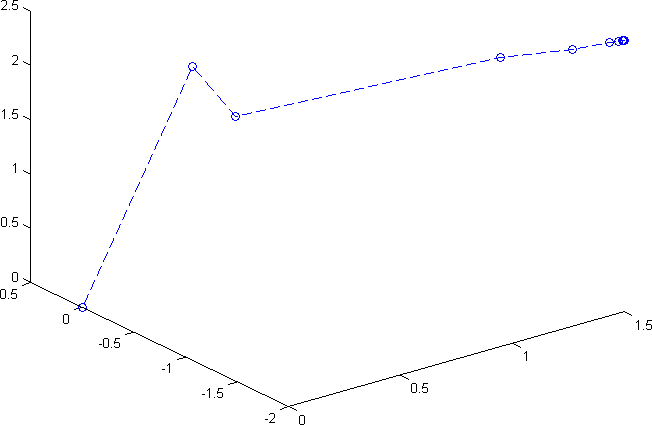
\includegraphics[width=0.5\textwidth]{img/SOR_3D_8_It_w_1_27.png}
	\caption{SOR, 8 Iterationen, $\omega=1.27=\omega_{\text{opt}}$}
	\label{fig:SOR w=1.27 3D Bsp}
\end{figure}
\begin{figure}[!ht]\centering
%	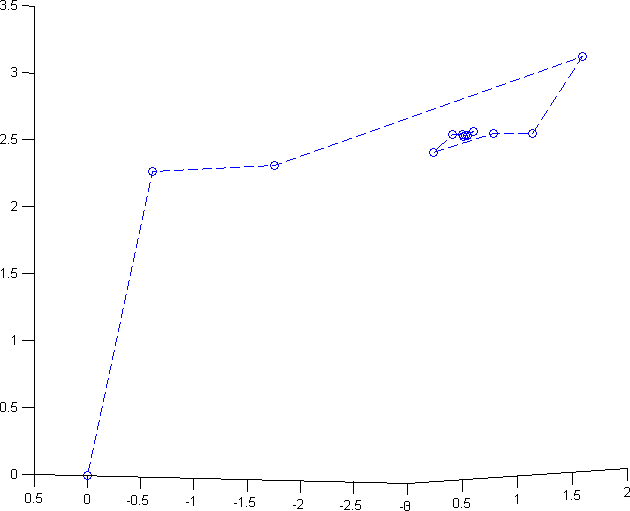
\includegraphics[width=0.5\textwidth]{img/SOR_3D_19_It_w_1_6.png}
	\caption{SOR, 19 Iterationen, $\omega=1.6$}
	\label{fig:SOR w=1.6 3D Bsp}
\end{figure}
			
\section{SSOR-Prinzip}
\index{SSOR}
\index{Symmetric SOR}
``Symmetric SOR'' ist eine Erweiterung des in Kapitel \ref{sec: SOR-Alg.}
beschriebenen SOR-Algorithmus. In einem einzelnen Iterationsschritt
folgt bei SSOR auf den in Gleichung (\ref{eq: SOR-It.formel1})
beschriebenen ``Vorw"arts-Schritt'' von SOR (mit $i=1,\ ...,\ n$) nun
noch ein zus"atzlicher Schritt, bei dem die Vektor-Komponenten $x_i$ in
umgekehrter Reihenfolge (also mit $i=n,\ ...,\ 1$) berechnet werden. Dies
f"uhrt somit zu dem folgenden, vollst"andigen SSOR-Iterationsschritt
f"ur den Gauss-Seidel-Algorithmus (vergleiche dazu Kapitel \ref{subsec:
SOR-Herleitung}, Gleichung \ref{eq: SOR-It.formel}):
\begin{equation} \label{eq: SSOR-It.formel-k+1/2}
	x^{(k+\frac{1}{2})}=(D+\omega L)^{-1}\cdot(\omega b-[\omega U+(\omega-1)\cdot D]\cdot x^{(k)})
\end{equation}
\begin{equation} \label{eq: SSOR-It.formel-k+1}
	x^{(k+1)}=(D+\omega U)^{-1}\cdot(\omega b-[\omega L+(\omega-1)\cdot D]\cdot x^{(k+\frac{1}{2})})
\end{equation}
Dabei nutzt man aus, dass der Gauss-Seidel-Algorithmus -- im Gegensatz
zum simultanen Jacobi-Algorithmus -- sukzessive ist. Das heisst, die
Resultate der einzelnen $x_i$ sind abh"angig von der Reihenfolge derer
Berechnung, da bei Gauss-Seidel jedes $x_i$ mit $i>1$ (bzw. in Gleichung
\ref{eq: SSOR-It.formel-k+1} mit $i<n$) abh"angig von im aktuellen
Iterationsschritt bereits berechneten $x_i$ ist. Deshalb auch der Name
``\textbf{Successive} Overrelaxation''.

W"urde man das SSOR-Prinzip auf den Jacobi-Algorithmus anwenden, so k"ame
dies zwei gew"ohnlichen SOR-Iterationsschritten gleich, da bei Jacobi
noch zu berechnende $x_i$ unabh"angig von im aktuellen Iterationsschritt
bereits berechneten $x_i$ sind.

Es soll an dieser Stelle erw"ahnt sein, dass SSOR "ublicherweise keine
Effizienzsteigerung gegen"uber SOR bietet. Die Konvergenz ist meist sogar
schlechter als mit SOR. Der Einsatz des SSOR-Verfahrens dient deshalb
eher der Vorkonditionierung \cite{Vorkonditionierung_Dorn} eines Problems
(sogenannter ``Preconditioner''). Dies bezeichnet die Umwandlung des
eigentlichen Ausgangsproblems in ein effizienter l"osbares Problem, zum
Beispiel f"ur nicht station"are iterative Verfahren. Die Ausgangsmatrix
soll auf diese Weise dahingehend vorbereitet werden, dass sich in der
weiteren Verarbeitung durch Vereinfachungsmethoden f"ur schwach besetzte
Matrizen m"oglichst Vorteile ergeben (verbesserte Spektraleigenschaften),
nicht jedoch die eigentliche L"osung des Systems beeinflusst wird.
\index{Preconditioner}
\index{Vorkonditionierung}

\printbibliography[heading=subbibliography]
\end{refsection}
